% 图 53.3 —— 由 `checks/emit_hand.py` 自动拼出（probe 精测 + prims2 图元分解）
%%
% ⚠ 这是**稿子不是成品**：跑 `checks/checkhand.py 53.3` 看指标 + 看叠合图。
%%
%% ⚠ 待核：
%   · 本图 probe 报出阴影族 1 个 —— **本脚本不生成阴影**（要照原书手写）；prims2 的 strokes 里可能含阴影线，核对时留意别画重
%   · 可疑字形 1 项（空心圈 ⊙ 常被认成字母 o）—— 见文件末
%%
\documentclass[12pt]{standalone}
\usepackage{fontspec}
\setsansfont{Arial}
\newfontfamily\mfallback{DejaVu Sans}
\usepackage{tikz}
\begin{document}
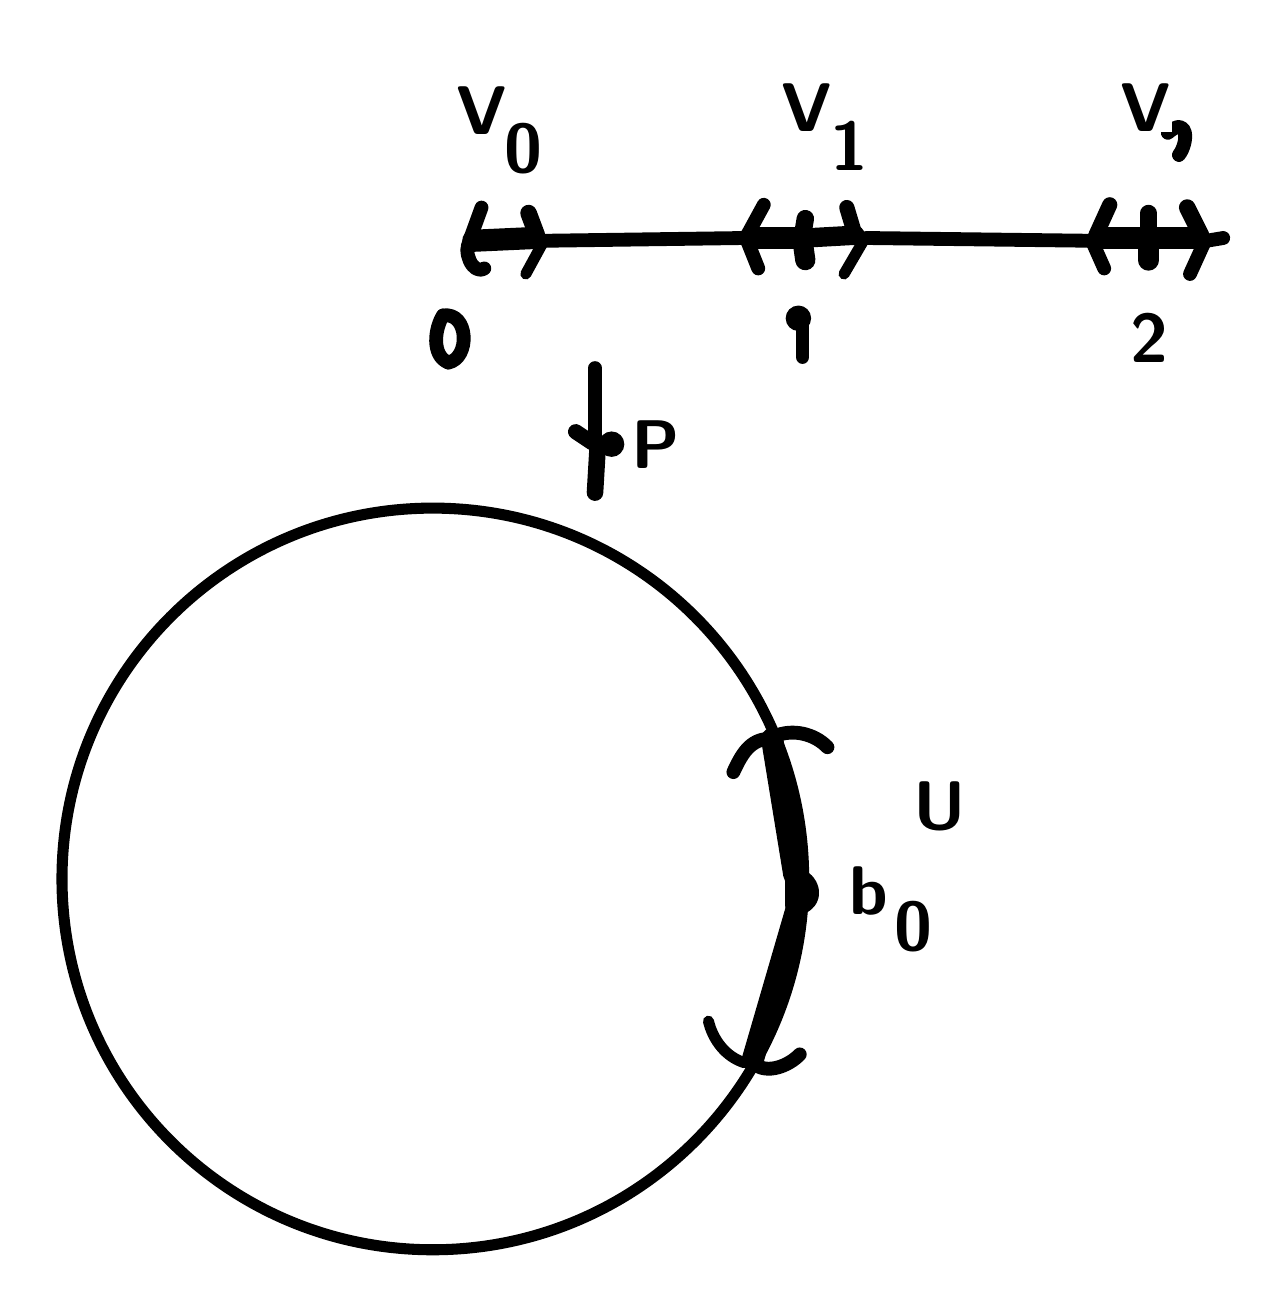
\begin{tikzpicture}[x=1pt, y=-1pt, line width=4.0pt, line cap=round, line join=round]

  %% ════ 填充区（prims2 的 fills）════

  %% ════ 直线段（prims2 的 strokes）════
  \draw[line width=6.3pt] (280.0,75.0) -- (281.0,69.0);
  \draw[line width=5.0pt] (426.0,77.0) -- (432.0,76.0);
  \draw[line width=8.0pt] (406.0,76.0) -- (423.0,76.0);
  \draw[line width=4.0pt] (180.0,89.0) -- (186.0,78.0);
  \draw[line width=5.0pt] (164.0,65.0) -- (160.0,76.0);
  \draw[line width=5.5pt] (391.0,64.0) -- (386.0,75.0);
  \draw[line width=7.0pt] (277.0,307.0) -- (277.0,317.0);
  \draw[line width=5.5pt] (198.0,146.0) -- (204.0,150.0);
  \draw[line width=5.0pt] (205.0,123.0) -- (205.0,149.0);
  \draw[line width=4.0pt] (302.0,77.0) -- (295.0,89.0);
  \draw[line width=8.0pt] (269.0,257.0) -- (277.0,306.0);
  \draw[line width=5.0pt] (303.0,76.0) -- (384.0,77.0);
  \draw[line width=7.6pt] (405.0,77.0) -- (405.0,84.0);
  \draw[line width=6.0pt] (405.0,75.0) -- (405.0,67.0);
  \draw[line width=5.0pt] (385.0,78.0) -- (389.0,87.0);
  \draw[line width=5.5pt] (296.0,65.0) -- (299.0,75.0);
  \draw[line width=6.0pt] (205.0,168.0) -- (206.0,151.0);
  \draw[line width=8.0pt] (278.0,318.0) -- (262.0,373.0);
  \draw[line width=5.0pt] (259.0,76.0) -- (187.0,77.0);
  \draw[line width=8.0pt] (387.0,76.0) -- (404.0,76.0);
  \draw[line width=5.0pt] (264.0,87.0) -- (260.0,77.0);
  \draw[line width=5.0pt] (280.0,119.0) -- (280.0,107.0);
  \draw[line width=6.0pt] (419.0,65.0) -- (424.0,75.0);
  \draw[line width=6.0pt] (181.0,67.0) -- (184.0,75.0);
  \draw[line width=8.0pt] (183.0,76.0) -- (161.0,77.0);
  \draw[line width=5.0pt] (266.0,64.0) -- (260.0,75.0);
  \draw[line width=8.0pt] (261.0,76.0) -- (279.0,76.0);
  \draw[line width=7.0pt] (299.0,75.0) -- (281.0,76.0);
  \draw[line width=7.3pt] (280.0,77.0) -- (281.0,84.0);
  \draw[line width=5.0pt] (425.0,78.0) -- (420.0,89.0);

  %% ════ 曲线（prims2 的 curves —— 三段式，坐标同为 (y,x)）════
  \draw[line width=5.0pt] (255.0,269.0) .. controls (257.7,263.2) and (260.8,257.0) .. (268.0,257.0);
  \draw[line width=7.0pt] (279.0,317.0) .. controls (284.6,315.1) and (282.9,308.6) .. (278.0,307.0);
  \draw[line width=5.0pt] (270.0,256.0) .. controls (276.3,253.3) and (284.2,255.0) .. (289.0,260.0);
  \draw[line width=5.0pt] (262.0,374.0) .. controls (266.9,378.6) and (275.1,375.1) .. (279.0,371.0);
  \draw[line width=4.0pt] (246.0,359.0) .. controls (247.6,365.7) and (252.2,371.9) .. (259.0,374.0);
  \draw[line width=5.0pt] (160.0,77.0) .. controls (156.9,80.1) and (160.7,89.7) .. (165.0,87.0);
  \draw[line width=5.0pt] (416.0,46.0) .. controls (419.5,41.5) and (419.5,31.5) .. (412.0,38.0);
  \draw[line width=5.0pt] (152.0,121.0) .. controls (145.8,118.5) and (147.1,108.5) .. (150.1,104.0);
  \draw[line width=5.0pt] (150.1,104.0) .. controls (159.5,102.6) and (159.9,119.5) .. (152.0,121.0);

  %% ════ 圆 / 椭圆（probe 精测）════
  \draw (146.4,307.6) circle (134.0);

  %% ════ 实心点 ════
  \fill (278.5,105.0) circle (4.6);
  \fill (211.0,150.5) circle (4.6);

  %% ════ 标签（probe 直接给的 \node 行）════
  %% ⚠ 全部补了 fill=white：文字在最上层，否则与曲线交叉干扰
     \node[anchor=center,inner sep=0pt,fill=white,font=\fontsize{28.8}{36.0}\selectfont] at (281.8,29.0) {\textsf{\textbf{\textit{V}}}};   % box(273,17,18,22)
     \node[anchor=center,inner sep=0pt,fill=white,font=\fontsize{28.0}{35.0}\selectfont] at (404.3,28.9) {\textsf{\textbf{\textit{V}}}};   % box(396,17,17,22)
     \node[anchor=center,inner sep=0pt,fill=white,font=\fontsize{28.0}{35.0}\selectfont] at (164.3,29.9) {\textsf{\textbf{\textit{V}}}};   % box(156,18,17,22)
     \node[anchor=center,inner sep=0pt,fill=white,font=\fontsize{24.5}{30.6}\selectfont] at (296.9,42.9) {\textsf{\textbf{1}}};   % box(290,34,8,17)
     \node[anchor=center,inner sep=0pt,fill=white,font=\fontsize{24.9}{31.1}\selectfont] at (179.1,43.7) {\textsf{\textbf{0}}};   % box(171,35,12,17)
     \node[anchor=center,inner sep=0pt,fill=white,font=\fontsize{31.4}{39.3}\selectfont] at (405.3,112.5) {\textsf{\textbf{2}}};   % box(397,101,15,22)
     \node[anchor=center,inner sep=0pt,fill=white,font=\fontsize{29.8}{37.3}\selectfont] at (227.0,150.5) {\textsf{\textbf{\textit{P}}}};   % box(216,138,18,23)
     \node[anchor=center,inner sep=0pt,fill=white,font=\fontsize{28.9}{36.1}\selectfont] at (329.5,281.2) {\textsf{\textbf{\textit{U}}}};   % box(320,269,19,22)
     \node[anchor=center,inner sep=0pt,fill=white,font=\fontsize{30.7}{38.3}\selectfont] at (303.8,311.8) {\textsf{\textbf{\textit{b}}}};   % box(294,299,17,23)
     \node[anchor=center,inner sep=0pt,fill=white,font=\fontsize{24.9}{31.1}\selectfont] at (320.1,324.7) {\textsf{\textbf{0}}};   % box(312,316,12,17)

  % 钉死画布：否则超出的图元/控制点会把页面撑大，1:1 回比就失准
  \pgfresetboundingbox
  \path[use as bounding box] (0,0) rectangle (441,452);
\end{tikzpicture}
\end{document}

% ⚠ 待核清单（probe 拿不准，人眼过一遍）：
%   · 未识别/跳过：⑤ 跳过/未识别的字形
